
\section{笛卡尔积的 Leibniz 稳定性}\label{sec:leibniz-stability-cartesian-products}

现在我们把注意力转向相对于\trCartesianProduct{}定义的类似 Leibniz 构造——
在\trMarkedSimplicialSet{}的语境中，它在 \cite{bib129} 中被称作\emph{Gray
张量积}（Gray tensor product）。我们先以一个关于\trLeibnizProduct{}之几何的基础
结果作为热身。

\begin{lemma}\label{lem:leibniz-product-mono}
\trSimplicialSet{}的任意一对\trMonomorphism{}的\trLeibnizProduct{}是一个%
\trMonomorphism。
\end{lemma}

\begin{proof}
诸\trProduct、诸\trPushout{}与诸\trMonomorphism{}都是在集合的\trCategory{}%
中逐点确定的，故此结果由下述事实得出：对集合的\trMonomorphism{}
$S\hookrightarrow T$ 与 $U\hookrightarrow V$，\trLeibnizProduct
\[ (S\hookrightarrow T)\mathbin{\widehat{\times}}(U\hookrightarrow V)
   \cong\bigl(S\times V\underset{S\times U}{\cup}T\times U
   \hookrightarrow T\times V\bigr) \]
是一个\trMonomorphism——逐一检视即明。
\end{proof}

\begin{remark}[为何称作「Leibniz」]\label{rem:why-leibniz}
由一对\trSimplex{}\trBoundary{}包含的\trLeibnizProduct{}所定义的包含
\begin{multline*}
(\partial\Delta[n]\hookrightarrow\Delta[n])\mathbin{\widehat{\times}}
(\partial\Delta[m]\hookrightarrow\Delta[m])\cong\\
\partial\Delta[n]\times\Delta[m]
\underset{\partial\Delta[n]\times\partial\Delta[m]}{\cup}
\Delta[n]\times\partial\Delta[m]\hookrightarrow\Delta[n]\times\Delta[m]
\end{multline*}
在几何上对应于\trPrism{}的\trBoundary{}
$\partial(\Delta[n]\times\Delta[m])\hookrightarrow\Delta[n]\times\Delta[m]$
这一包含。而等同
\[ \partial(\Delta[n]\times\Delta[m])\cong
   \partial\Delta[n]\times\Delta[m]
   \underset{\partial\Delta[n]\times\partial\Delta[m]}{\cup}
   \Delta[n]\times\partial\Delta[m] \]
在形式上类似于通常称作「Leibniz 法则」的种种恒等式。
\end{remark}

为证明一个关于\trMarkedSimplicialSet{}的类似结果，我们首先需要下述观察：

\begin{proposition}\label{prop:marked-cartesian-closed}
\trMarkedSimplicialSet{}的\trCategory{}是\trCartesianClosed，其中
\begin{itemize}
\item \trCartesianProduct{}定义如下：底\trSimplicialSet{}的%
  \trCartesianProduct{}中的一个\trSimplex{}被标记，当且仅当它的两个分量
  都是带标记\trSimplex；
\item \trInternalHom{} $Y^{X}$ 定义为这样一个\trSimplicialSet：其诸
  $n$-\trSimplex{}是\trMarkedSimplicialSet{}的映射
  $\sigma\colon X\times\Delta[n]\to Y$，而 $\sigma$ 被标记，当且仅当该
  映射可\trExtension{}为一个\trMarkedSimplicialSet{}的映射：
\begin{center}
\begin{tikzpicture}[x=1.8em,y=1.5em]
  \node (xt) at (0,1.3) {$X\times\Delta[n]$};
  \node (y) at (4.4,1.3) {$Y$};
  \node (xe) at (0,-1.1) {$X\times\Delta[n]_{t}$};
  \draw[->] (xt) -- node[above]{$\scriptstyle\sigma$} (y);
  \draw[right hook->] (xe) -- node[left]{$\scriptstyle e$} (xt);
  \draw[->,dashed] (1.1,-0.85) -- (3.7,0.95);
  \node at (2.2,0.25) {$\scriptstyle\sigma$};
\end{tikzpicture}
\end{center}
\end{itemize}
\end{proposition}

\begin{proof}
由\trProduct{}的\trUniversalProperty{}及其封闭性，显然：若这些对象存在，
\trCartesianProduct{}与\trInternalHom{}就必定以这种方式来定义。为验证这一%
\trAdjunction，回顾\cref{prop:reflective-embedding}：\trMarkedSimplicialSet{}%
作为反射全子范畴嵌入预层\trCategory{}
$\mathcal{S}et^{t\Delta^{\mathrm{op}}}$ 之中。由附录 A 中的%
\cref{exa:cartesian-closed-examples}，\trCategory{}
$\mathcal{S}et^{t\Delta^{\mathrm{op}}}$ 是\trCartesianClosed，而且这一
嵌入保持刚才定义的诸\trProduct{}与诸\trInternalHom{}。于是我们得出结论：
把相应的自然\trIsomorphism{}从 $\mathcal{S}et^{t\Delta^{\mathrm{op}}}$
限制到其全子范畴上，这些数据便定义了 $\sSet^{+}$ 上一个双变量\trAdjunction{}%
的诸\trFunctor。
\end{proof}

\cref{lem:leibniz-product-mono}的结果可以扩张到带标记的语境。我们的证明用到
一条也在别处被调用的简单观察。

\begin{lemma}\label{lem:leibniz-entire}
\trMarkedSimplicialSet{}的任一映射与一个\trEntireInclusion{}的\trLeibnizProduct{}是一个\trEntireInclusion。
\end{lemma}

\begin{proof}
按定义，$f\colon X\to Y$ 与 $i\colon U\hookrightarrow_{e}V$ 的\trLeibnizProduct{}是
如下所诱导的\trMarkedSimplicialSet{}的映射
\begin{center}
\begin{tikzpicture}[x=1.8em,y=1.5em]
  \node (xu) at (0,1.9) {$X\times U$};
  \node (xv) at (3.6,1.9) {$X\times V$};
  \node (yu) at (0,0.2) {$Y\times U$};
  \fill (3.0,0.2) circle (1.1pt);
  \node at (2.62,0.55) {$\scriptstyle\ulcorner$};
  \node (yv) at (4.6,-1.7) {$Y\times V$};
  \draw[right hook->] (xu) -- node[above]{$\scriptstyle X\times i$} node[pos=0.2,below]{$\scriptstyle e$} (xv);
  \draw[->] (0,1.55) -- (0,0.6);
  \node at (-0.8,1.05) {$\scriptstyle f\times U$};
  \draw[->] (3.6,1.55) -- (3.05,0.55);
  \draw[->] (0.75,0.2) -- (2.55,0.2);
  \node at (1.65,-0.2) {$\scriptstyle\hookrightarrow_{e}$};
  \draw[->,dashed] (3.15,-0.1) -- (4.3,-1.35);
  \draw[->] (3.95,1.6) .. controls (5.5,0.9) and (5.6,-0.6) .. (5.15,-1.55);
  \node at (5.6,0.15) {$\scriptstyle f\times V$};
  \draw[->] (0.55,-0.15) .. controls (2.0,-1.15) and (3.4,-1.7) .. (3.9,-1.72);
  \node at (1.7,-1.2) {$\scriptstyle Y\times i$};
  \node at (4.05,-2.05) {$\scriptstyle\hookrightarrow_{e}$};
\end{tikzpicture}
\end{center}
注意\trForgetfulFunctor{} $(-)_{0}\colon\sSet^{+}\to\sSet$ 保持诸%
\trProduct{}与诸\trPushout，并回顾：\trMarkedSimplicialSet{}的一个映射是%
\trEntireInclusion，当且仅当其底映射是一个\trIsomorphism。由于一个\trSimplicialSet{}%
与一个\trIsomorphism{}的\trProduct{}是\trIsomorphism，映射
$X\times U\hookrightarrow_{e}X\times V$ 与
$Y\times U\hookrightarrow_{e}Y\times V$ 都是\trEntireInclusion。又由于诸%
\trIsomorphism{}的\trPushout{}是\trIsomorphism，剩下那条水平映射也是%
\trEntireInclusion。最后，由于诸\trIsomorphism{}满足\trTwoOfThreeProperty，\trLeibnizProduct
映射必定也是\trEntireInclusion。
\end{proof}

\begin{lemma}\label{lem:leibniz-regular}
两个正则包含的\trLeibnizProduct{}仍是正则包含。
\end{lemma}

\begin{proof}
由\cref{lem:leibniz-product-mono}，两个正则包含
$A\hookrightarrow_{r}B$ 与 $C\hookrightarrow_{r}D$ 的\trLeibnizProduct{}之底%
\trSimplicialSet{}是\trMonomorphism
\[ A\times D\underset{A\times C}{\cup}B\times C
   \hookrightarrow B\times D\mbox{.} \]
特别地，注意分量 $A\times D$ 与 $B\times C$ 的诸包含联合满地映到该映射的
定义域上。我们的任务是证明：$A\times D\underset{A\times C}{\cup}B\times C$
中任何一个在 $B\times D$ 中被标记的 $n$-\trSimplex{}，在
$A\times D\underset{A\times C}{\cup}B\times C$ 中也被标记。我们分情形
论证，并不失一般性假设该 $n$-\trSimplex{}位于来自 $B\times C$ 的包含的像
之中。此时，映射 $B\times C\hookrightarrow_{r}B\times D$ 的正则性蕴含：
它在 $A\times D\underset{A\times C}{\cup}B\times C$ 中被标记，正如所断言。
\end{proof}

\trMarkedSimplicialSet{}的一个一般\trMonomorphism{}既非正则包含亦非\trEntireInclusion，
但\trMarkedSimplicialSet{}的诸生成\trMonomorphism{}却具有这两种性质之一。
于是，由\cref{lem:leibniz-entire}与\cref{lem:leibniz-regular}，我们立即
得出：

\begin{lemma}\label{lem:leibniz-generating}
对任意 $n,m\ge 0$，诸\trLeibnizProduct
\begin{gather*}
(\partial\Delta[n]\hookrightarrow_{r}\Delta[n])\mathbin{\widehat{\times}}
(\partial\Delta[m]\hookrightarrow_{r}\Delta[m]),\qquad
(\partial\Delta[n]\hookrightarrow_{r}\Delta[n])\mathbin{\widehat{\times}}
(\Delta[m]\hookrightarrow_{e}\Delta[m]_{t}),\\
\text{以及}\qquad
(\Delta[n]\hookrightarrow_{e}\Delta[n]_{t})\mathbin{\widehat{\times}}
(\Delta[m]\hookrightarrow_{e}\Delta[m]_{t})
\end{gather*}
都是\trMarkedSimplicialSet{}的\trMonomorphism。
\end{lemma}

作为一个推论，我们可以借助一个在本章中反复出现的十分一般的论证来刻画%
\trMarkedSimplicialSet{}的任意\trMonomorphism{}的\trLeibnizProduct。

\begin{corollary}\label{cor:leibniz-mono-tf}
\begin{enumerate}[label=(\roman*)]
\item \trMarkedSimplicialSet{}的任意一对\trMonomorphism{}的\trLeibnizProduct{}仍是
  一个\trMonomorphism。
\item \trMarkedSimplicialSet{}的任一\trTrivialFibration{}与任一%
  \trMonomorphism{}的 Leibniz 指数（Leibniz exponential）仍是一个%
  \trTrivialFibration。
\end{enumerate}
\end{corollary}

\begin{proof}
以\cref{lem:leibniz-two-variable-adjunction}的术语来说，这两条陈述合起来
断言：由\trCartesianProduct{}与\trInternalHom{}定义的双变量\trAdjunction{}%
相对于（\trMonomorphism，\trTrivialFibration）这一%
\trWeakFactorizationSystem{}是一个 Leibniz 双变量\trAdjunction。由
\cref{rem:leibniz-generators}，这可由
\cref{lem:mono-marked-cellularly-generated}与\cref{lem:leibniz-generating}
所建立的性质得出。
\end{proof}

困难得多的是证明：带标记\trAnodyneExtension{}类对于带标记\trMonomorphism{}类具有
Leibniz 稳定性。我们证明一个略更具体的结果，它同时刻画了内、左或右带标记%
\trAnodyneExtension{}的情形——这些情形分别把不等式 $0\le k\le n$ 限制为 $0<k<n$、
$k<n$ 或 $0<k$。

\begin{proposition}\label{prop:leibniz-marked-anodyne}
对 $n\ge 1$、$m\ge 0$ 且 $0<k\le n$，下列\trLeibnizProduct{}中的每一个都是右带标记%
\trAnodyneExtension，并且当 $k<n$ 时是内带标记\trAnodyneExtension：
\begin{gather*}
(\Lambda^{k}[n]\hookrightarrow_{r}\Delta^{k}[n])\mathbin{\widehat{\times}}
(\partial\Delta[m]\hookrightarrow_{r}\Delta[m])\\
(\Lambda^{k}[n]\hookrightarrow_{r}\Delta^{k}[n])\mathbin{\widehat{\times}}
(\Delta[m]\hookrightarrow_{e}\Delta[m]_{t})\\
(\Delta^{k}[n]'\hookrightarrow_{e}\Delta^{k}[n]'')\mathbin{\widehat{\times}}
(\partial\Delta[m]\hookrightarrow_{r}\Delta[m])\\
(\Delta^{k}[n]'\hookrightarrow_{e}\Delta^{k}[n]'')\mathbin{\widehat{\times}}
(\Delta[m]\hookrightarrow_{e}\Delta[m]_{t})
\end{gather*}
\end{proposition}

鉴于\trCartesianProduct{}的对称性，\trHorn{}包含与\trSimplex{}\trBoundary{}%
包含何者居左、何者居右并无分别。这一结果的证明需要某些特殊记号来描述%
\trSimplex{}的\trCartesianProduct。

\begin{digression}[论洗牌]\label{dig:on-shuffles}
由于 $\Delta[n]$ 是偏序集（poset）$[n]$ 的\trNerve，一个 $r$-\trSimplex{}
$i\colon\Delta[r]\to\Delta[n]$ 同样可以由出现于其像中的顶点的有序序列
$i_{0}\le\cdots\le i_{r}\in[n]$ 来编码。

由\trProduct{}的\trUniversalProperty，$\Delta[n]\times\Delta[m]$ 中的一个
$r$-\trSimplex{}由一个 $r$-\trSimplex{} $i\colon\Delta[r]\to\Delta[n]$ 与一个
$r$-\trSimplex{} $j\colon\Delta[r]\to\Delta[m]$ 给出。由于
$\Delta[n]\times\Delta[m]$ 是偏序集 $[n]\times[m]$ 的\trNerve，这样的%
\trSimplex{}与由二元组构成的有序序列
\begin{rveq}\label{eq:pair-sequence}
(i_{0},j_{0})\le(i_{1},j_{1})\le\cdots\le(i_{r},j_{r})
\end{rveq}
一一对应，其中每个 $i_{s}\in[n]$、每个 $j_{t}\in[m]$；而且它退化，当且仅当
这些不等式中的某一个是等式。

\trSimplicialSet{} $\Delta[n]\times\Delta[m]$ 的非退化
$(n+m)$-\trSimplex{}称作\textbf{洗牌}（shuffles）；它们是具有最高维数的%
\trSimplex。一个 $(n+m)$-\trSimplex{} $(i,j)$ 定义一个洗牌，当且仅当对一切
$t\in[n+m]$ 都有 $i_{t}+j_{t}=t$。若把 $[n]\times[m]$ 的对象排布成一个
矩形网格，洗牌便是那些从 $(0,0)$ 出发、以 $(n,m)$ 收尾的极大长度非退化
路径——每一步恰给某一个坐标加一。
\end{digression}

下面证明的第一个情形，是把 Dugger 与 Spivak 的一个论证 \cite[A.1]{bib36}
改编到带标记的语境。

\begin{proof}[\cref{prop:leibniz-marked-anodyne}的证明]
由\cref{lem:leibniz-regular}，\trLeibnizProduct{}
$(\Lambda^{k}[n]\hookrightarrow_{r}\Delta^{k}[n])\mathbin{\widehat{\times}}(\partial\Delta[m]\hookrightarrow_{r}\Delta[m])$ 是正则包含
\[ \Lambda^{k}[n]\times\Delta[m]
   \underset{\Lambda^{k}[n]\times\partial\Delta[m]}{\cup}
   \Delta^{k}[n]\times\partial\Delta[m]
   \hookrightarrow_{r}\Delta^{k}[n]\times\Delta[m]\mbox{.} \]
一个非退化 $r$-\trSimplex{} \eqref{eq:pair-sequence} 于
$\Delta^{k}[n]\times\Delta[m]$ 中不在这个\trLeibnizProduct{}包含的定义域内，当且仅当%
\yizhu{原书于此印作「of $\Lambda^{k}[n]\times\Delta[m]$」，然该并集之定义域
本就包含 $\Lambda^{k}[n]\times\Delta[m]$，其中的\trSimplex{}无从「缺失」；
按文义应为余域 $\Delta^{k}[n]\times\Delta[m]$ 之误，此处径改。——译者注}
\begin{itemize}
\item 它的分量 $\{i_{0},\dots,i_{r}\}\supseteq[n]\setminus\{k\}$，并且
\item 它的分量 $\{j_{0},\dots,j_{r}\}\supseteq[m]$。
\end{itemize}
我们将这一包含过滤成一列正则包含
\[ \Lambda^{k}[n]\times\Delta[m]
   \underset{\Lambda^{k}[n]\times\partial\Delta[m]}{\cup}
   \Delta^{k}[n]\times\partial\Delta[m]=:Y^{-1}
   \hookrightarrow_{r}\cdots\hookrightarrow_{r}Y^{m}
   =\Delta^{k}[n]\times\Delta[m] \]
并论证：视情形而定，每个 $Y^{t}\hookrightarrow Y^{t+1}$ 都是右或内带标记%
\trAnodyne{}的。

从 $Y^{-1}:=\Lambda^{k}[n]\times\Delta[m]\underset{\Lambda^{k}[n]\times\partial\Delta[m]}{\cup}\Delta^{k}[n]\times\partial\Delta[m]$ 出发，我们把 $Y^{t}$ 定义为
$\Delta^{k}[n]\times\Delta[m]$ 的这样一个最小的正则单纯子集：它包含
$Y^{t-1}$ 以及每一个含有顶点 $(k,t)$ 的\trSimplex{}
\eqref{eq:pair-sequence}。由于每一个缺失的\trSimplex{}都是含有顶点
$(k,0),\dots,(k,m)$ 之一的某个\trSimplex{}的一个面，从此描述即清楚可见
$Y^{m}=\Delta^{k}[n]\times\Delta[m]$。

剩下的只是分析诸正则包含 $Y^{t-1}\hookrightarrow_{r}Y^{t}$，我们通过给出
另一重过滤来做到这一点：
\[ Y^{t-1}=Y^{t,n-1}\hookrightarrow_{r}Y^{t,n}\hookrightarrow_{r}
   \cdots\hookrightarrow_{r}Y^{t,n+m}=Y^{t}\mbox{.} \]

注意：$\Delta^{k}[n]\times\Delta[m]$ 中含有顶点 $(k,t)$ 且维数不超过 $n-1$
的\trSimplex{}都含于 $Y^{-1}$，因此那些含有顶点 $(k,t)$、附着到 $Y^{t-1}$
上以构成 $Y^{t}$ 的\trSimplex{}，其维数介于 $n$ 与 $n+m$ 之间。有鉴于此，
我们把 $Y^{t,r}$ 定义为 $\Delta^{k}[n]\times\Delta[m]$ 的包含 $Y^{t,r-1}$
与一切含有顶点 $(k,t)$ 的 $r$ 维\trSimplex{}的最小正则单纯子集。特别地，
$Y^{t,n-1}=Y^{t-1}$ 而 $Y^{t,n+m}=Y^{t}$。

我们现在论证：这一过滤中的每个正则包含都先是一个由诸复状号角扩张之余积
构成的推出，继而是诸复状薄性扩张之余积的推出
\begin{center}
\begin{tikzpicture}[x=1.9em,y=1.5em]
  \node (lam) at (0,2.6) {$\coprod_{\tau\in S^{t,r}}\Lambda^{\ell_{\tau}}[r]$};
  \node (ytr1) at (6.4,2.6) {$Y^{t,r-1}$};
  \node (dl) at (0,0) {$\coprod_{\tau\in S^{t,r}}\Delta^{\ell_{\tau}}[r]$};
  \fill (4.0,0) circle (1.1pt);
  \node at (3.62,0.35) {$\scriptstyle\lrcorner$};
  \node (dr) at (9.2,0) {$\coprod_{\tau\in T^{t,r}}\Delta^{\ell_{\tau}}[r]'$};
  \node (ytr) at (4.0,-2.6) {$Y^{t,r}$};
  \node (dd) at (9.2,-2.6) {$\coprod_{\tau\in T^{t,r}}\Delta^{\ell_{\tau}}[r]''$};
  \draw[->] (lam) -- (ytr1);
  \draw[right hook->] (0,2.1) -- node[left]{$\scriptstyle r$} (0,0.55);
  \draw[right hook->] (6.4,2.05) -- (4.15,0.4);
  \draw[->] (1.9,0) -- (3.6,0);
  \draw[->] (7.5,0) -- (4.4,0);
  \draw[right hook->] (9.2,0.55) -- node[right]{$\scriptstyle e$} (9.2,-2.05);
  \draw[right hook->] (4.0,-0.55) -- node[left]{$\scriptstyle e$} (4.0,-2.05);
  \node at (3.62,-2.2) {$\scriptstyle\lrcorner$};
  \draw[->] (7.5,-2.6) -- (4.8,-2.6);
\end{tikzpicture}
\end{center}
其由集合 $S^{t,r}$——含有顶点 $(k,t)$ 且尚未出现在 $Y^{t,r-1}$ 中的
$r$-\trSimplex{}之集——标引，而 $T^{t,r}\subset S^{t,r}$ 则定义为那些使
$\tau\delta^{\ell_{\tau}}$ 在 $\Delta^{k}[n]\times\Delta[m]$ 中被标记的
$r$-\trSimplex{} $\tau$ 组成的子集。此外，对每个 $\tau\in S^{t,r}$，我们将
看到 $0<\ell_{\tau}$，而当 $k<n$ 时 $\ell_{\tau}<r$。这将表明：该\trLeibnizProduct
是一个右带标记\trAnodyneExtension，并且当 $k<n$ 时是一个内带标记\trAnodyneExtension。

为看到这一点，设 $\tau\in S^{t,r}$ 是 $r$-\trSimplex{}
\[ (i_{0},j_{0})\le\cdots\le(i_{\ell_{\tau}},j_{\ell_{\tau}})=(k,t)
   \le\cdots\le(i_{r},j_{r}) \]
它以 $(k,t)$ 为其第 $\ell_{\tau}$ 个顶点；为便于阅读，下文将 $\ell_{\tau}$
写作 $\ell$。由于集合 $\{i_{0},\dots,i_{r}\}\supseteq[n]$ 且 $0<k$，必有
$0<\ell$；而若 $k<n$，亦必有 $\ell<r$。我们将论证：
\begin{itemize}
\item $\tau$ 的除第 $\ell$ 面之外的各个面都含于 $Y^{t,r-1}$；
\item $\tau$ 的第 $\ell$ 面不在 $Y^{t,r-1}$ 中；
\item $r$-\trSimplex{} $\tau$ 是 $\Delta^{k}[n]\times\Delta[m]$ 的一个
  $\ell$-容许\trSimplex；
\item 若 $\tau\delta^{\ell}$ 在 $\Delta^{k}[n]\times\Delta[m]$ 中被标记，
  则 $\tau\delta^{\ell-1}$ 与 $\tau\delta^{\ell+1}$（在 $\ell<r$ 的情形）
  亦然。
\end{itemize}
于是，$\tau$ 与 $Y^{t,r-1}$ 之并，可以如所断言地作为一个复状号角扩张
$\Lambda^{\ell}[r]\hookrightarrow_{r}\Delta^{\ell}[r]$ 的推出而构成。

对于第一条，注意除 $\tau\delta^{\ell}$ 之外的每个余维一面都具有维数 $r-1$
且含有顶点 $(k,t)$，从而如所断言地落在 $Y^{t,r-1}$ 中。为看出
$Y^{t,r-1}$ 并不同时包含面 $\tau\delta^{\ell}$，我们考虑顶点
$(i_{\ell-1},j_{\ell-1})$。若 $i_{\ell-1}=k$，则由非退化性有
$j_{\ell-1}<t$，此时将有 $\tau\in Y^{t-1}$，矛盾。故 $i_{\ell-1}<k$。又若
$i_{\ell-1}\le k-2$，则将有 $\tau\in Y^{-1}$，又生矛盾。于是必有
$i_{\ell-1}=k-1$。再若 $j_{\ell-1}<t$，则 $\tau$ 将是
\[ (i_{0},j_{0})\le\cdots\le(i_{\ell-1},j_{\ell-1})\le(k,t-1)
   \le(i_{\ell},j_{\ell})=(k,t)\le\cdots\le(i_{r},j_{r}) \]
这一 $(r+1)$ 维\trSimplex{}的一个面，而后者含于 $Y^{t-1}$，矛盾。所以我们
得出 $(i_{\ell-1},j_{\ell-1})=(k-1,t)$。

由这一计算我们看出，$\tau\delta^{\ell}$ 的顶点满足
$\{i_{0},\dots,i_{\ell-1}=k-1,i_{\ell+1},\dots,i_{r}\}\supseteq[n]\setminus\{k\}$ 与
$\{j_{0},\dots,j_{\ell-1},j_{\ell+1},\dots,j_{r}\}\supseteq[m]$。于是
$\tau\delta^{\ell}$ 不在 $Y^{-1}$ 中。此外，$\tau\delta^{\ell}$ 也没有在
通往 $Y^{t,r-1}$ 的途中被添入，因为它不是含有顶点 $(k,s)$（对任何 $s<t$）
的任何\trSimplex{}的面。这完成了我们的第二项任务。

我们已经证明：可以通过填充一个适当的号角，把 $\tau$ 连同其第 $\ell$ 面
附着到 $Y^{t,r-1}$ 上。剩下的只是论证：我们赖以附着 $\tau$ 的那个号角
$\Lambda^{\ell}[r]\to Y^{t,r-1}$ 是容许的。由于包含
$Y^{t,r-1}\hookrightarrow_{r}\Delta^{k}[n]\times\Delta[m]$ 是正则的，只需
证明：含有顶点 $(i_{\ell-1},j_{\ell-1})$、$(i_{\ell},j_{\ell})$ 与
$(i_{\ell+1},j_{\ell+1})$ 的每个\trSimplex{}——在 $\ell=r$ 的情形则只需
含有前两个顶点——都在 $\Delta^{k}[n]\times\Delta[m]$ 中被标记。上文已经
见到 $(i_{\ell-1},j_{\ell-1})=(k-1,t)$ 与 $(i_{\ell},j_{\ell})=(k,t)$。在
$\ell<r$ 的情形，由于 $\tau$ 在 $Y^{-1}$ 中缺失，$i_{\ell+1}$ 必等于 $k$
或 $k+1$。此时，该\trSimplex{}在 $\Delta[m]$ 中的分量是退化的，含有序列
$t\le t$；而其在 $\Delta^{k}[n]$ 中的分量要么是退化的，要么含有序列
$k-1\le k\le k+1$，要么——在 $\ell=r$（此时 $k=n$）的情形——含有序列
$k-1\le k$。于是两个分量都是带标记\trSimplex，这就是说，它们的%
\trProduct{}如所需地在 $\Delta^{k}[n]\times\Delta[m]$ 中被标记。

最后，我们必须论证：由推出附着的诸\trSimplex{}包含正则子集
$Y^{t,r}\hookrightarrow\Delta^{k}[n]\times\Delta[m]$ 中在场的一切标记。
出现在 $Y^{t,r}$ 中而不出现在 $Y^{t,r-1}$ 中的\trSimplex{}只在维数 $r$ 与
$r-1$。新附着的诸 $r$-\trSimplex{}都是带标记的，所以我们只需关心那个
$(r-1)$-\trSimplex{}
\[ (i_{0},j_{0})\le\cdots\le(i_{\ell-1},j_{\ell-1})=(k-1,t)
   \le(i_{\ell+1},j_{\ell+1})\le\cdots\le(i_{r},j_{r}) \]
——它对每个 $\tau\in S^{t,r}$ 作为其 $\ell$ 面出现，当该\trSimplex{}在
$\Delta^{k}[n]\times\Delta[m]$ 中被标记时。

分两种情形，视 $i_{\ell+1}=k+1$ 还是 $i_{\ell+1}=k$ 而定。在前一情形，
这个\trSimplex{}被标记这一事实告诉我们：序列
$i_{0}\le\cdots\le i_{\ell-1}\le i_{\ell+1}\le\cdots\le i_{r}$ 中存在一处
重复，并且序列
$j_{0}\le\cdots\le j_{\ell-1}\le j_{\ell+1}\le\cdots\le j_{r}$ 中亦然。当
我们把第一个序列中的 $i_{\ell-1}$ 或 $i_{\ell+1}$ 换成 $i_{\ell}=k$ 时，
该重复要么仍然保持，要么我们便得到子序列 $k-1\le k\le k+1$。无论何种
方式，这都告诉我们：诸面 $\tau\delta^{\ell-1}$ 与 $\tau\delta^{\ell+1}$
的这一分量在 $\Delta^{k}[n]$ 中被标记。类似地，当我们把 $j_{\ell}=t$ 换成
$j_{\ell-1}=t$ 时，序列不变；而当我们为 $j_{\ell+1}$ 作替换时，我们的序列
便含有一处重复 $t\le t$。无论何种方式，这都告诉我们：诸面
$\tau\delta^{\ell-1}$ 与 $\tau\delta^{\ell+1}$ 的这一分量在 $\Delta[m]$
中被标记。总而言之，\trSimplex{}
$\tau\colon\Delta^{\ell}[r]\to\Delta^{k}[n]\times\Delta[m]$ 沿
$\Delta^{k}[n]\hookrightarrow_{e}\Delta^{k}[n]'$ 容有\trExtension，于是
我们沿第二次推出中所包含的\trEntireInclusion
$\Delta^{k}[n]'\hookrightarrow_{e}\Delta^{k}[n]''$ 作\trExtension，便得到
其第 $\ell$ 面的所需标记。

在 $i_{\ell+1}=k$ 的情形，$\tau\delta^{\ell-1}$ 的顶点序列在其第一分量中
含有 $k\le k$，而在其第二分量中则与 $\tau\delta^{\ell}$ 的顶点序列相同。
于是 $\tau\delta^{\ell-1}$ 被标记。$\tau\delta^{\ell+1}$ 的顶点序列在其
第一分量中含有 $k-1\le k\le k+1$，在其第二分量中含有 $t\le t$。于是
$\tau\delta^{\ell+1}$ 被标记，而且我们再一次沿第二次推出中所包含的\trEntireInclusion
$\Delta^{k}[n]'\hookrightarrow_{e}\Delta^{k}[n]''$ 作\trExtension，便得到
其第 $\ell$ 面的所需标记。这就完成了「第一个\trLeibnizProduct{}是带标记%
\trAnodyneExtension」的证明。

由\cref{lem:leibniz-entire}，其余三个\trLeibnizProduct{}都是\trEntireInclusion，故所需做的
只是验证：余域中在场的附加标记都是诸复状薄性扩张的结果。我们把涉及%
\trLeibnizProduct
\[ (\Delta^{k}[n]'\hookrightarrow_{e}\Delta^{k}[n]'')
   \mathbin{\widehat{\times}}(A\hookrightarrow B) \]
的两种情形——即一个复状薄性扩张与一个带标记\trMonomorphism{}的\trLeibnizProduct
——同时处理。\yizhu{原书于此印作「of a complicial horn extension」（复状
号角扩张）；然所处理两情形之首因子均为复状薄性扩张
$\Delta^{k}[n]'\hookrightarrow_{e}\Delta^{k}[n]''$，且上句明言附加标记「都是诸
复状薄性扩张的结果」，按文义应为薄性扩张之误，此处径改。——译者注}$\Delta^{k}[n]''$ 中唯一一个在 $\Delta^{k}[n]'$ 中不被
标记的带标记\trSimplex{}是面
$\delta^{k}\colon\Delta[n-1]_{t}\to\Delta^{k}[n]''$，这意味着我们有拉回与
推出方块
\begin{center}
\begin{tikzpicture}[x=2.1em,y=1.6em]
  \node (tl) at (0,1.4) {$\coprod_{\tau\in S}\Delta[n-1]$};
  \node (tr) at (10.4,1.4)
    {$\Delta^{k}[n]'\times B\underset{\Delta^{k}[n]'\times A}{\cup}\Delta^{k}[n]''\times A$};
  \node (bl) at (0,-1.3) {$\coprod_{\tau\in S}\Delta[n-1]_{t}$};
  \node (br) at (10.4,-1.3) {$\Delta^{k}[n]''\times B$};
  \draw[->] (2.4,1.4) -- (5.2,1.4);
  \draw[right hook->] (0,0.85) -- (0,-0.7);
  \node at (-0.5,0.1) {$\scriptstyle e$};
  \draw[right hook->] (10.4,0.85) -- (10.4,-0.7);
  \node at (10.9,0.1) {$\scriptstyle e$};
  \draw[->] (2.9,-1.3) -- node[below]{$\scriptstyle(\delta^{k},\tau)$} (5.6,-1.3);
  \node at (2.15,1.05) {$\scriptstyle\ulcorner$};
  \node at (10.05,-0.95) {$\scriptstyle\lrcorner$};
\end{tikzpicture}
\end{center}
其中 $S$ 是 $B$ 中那些未在 $A$ 中出现或未在 $A$ 中被标记的带标记
$(n-1)$-\trSimplex{}之集。我们论证：对 $B$ 中任何带标记 $(n-1)$-\trSimplex{}
$\tau$，退化 $n$-\trSimplex{} $\tau\sigma^{k-1}$ 容有如下图式所示的诸标记：
\begin{center}
\begin{tikzpicture}[x=1.9em,y=1.5em]
  \node (tl) at (0,1.2) {$\Delta[n]$};
  \node (tr) at (4.6,1.2) {$\Delta^{k}[n]''$};
  \node (bl) at (0,-1.2) {$\Delta[n-1]_{t}$};
  \node (br) at (4.6,-1.2) {$B$};
  \draw[right hook->] (1.0,1.2) -- node[above]{$\scriptstyle e$} (3.3,1.2);
  \draw[->] (0,0.8) -- (0,-0.7);
  \node at (-0.9,0.05) {$\scriptstyle\sigma^{k-1}$};
  \draw[->] (1.0,-1.2) -- node[below]{$\scriptstyle\tau$} (3.3,-1.2);
  \draw[->>,dashed] (4.6,0.8) -- (4.6,-0.7);
\end{tikzpicture}
\end{center}
这是因为第 $k-1$ 面与第 $k$ 面都等于 $\tau$，从而被标记，而任何含有顶点
$k-1$ 与 $k$ 的面都是退化的，从而也被标记；这些条件覆盖了全部所需的带标记
面。现在清楚的是：上方的推出方块经由左侧的推出图式而分解
\begin{center}
\begin{tikzpicture}[x=1.7em,y=1.55em]
  \node (a) at (0,1.4) {$\coprod_{\tau\in S}\Delta[n-1]$};
  \node (b) at (5.6,1.4) {$\coprod_{\tau\in S}\Delta^{k}[n]'$};
  \node (c) at (14.6,1.4)
    {$\Delta^{k}[n]'\times B\underset{\Delta^{k}[n]'\times A}{\cup}\Delta^{k}[n]''\times A$};
  \node (d) at (0,-1.4) {$\coprod_{\tau\in S}\Delta[n-1]_{t}$};
  \node (e) at (5.6,-1.4) {$\coprod_{\tau\in S}\Delta^{k}[n]''$};
  \node (f) at (14.6,-1.4) {$\Delta^{k}[n]''\times B$};
  \draw[->] (2.2,1.4) -- (3.8,1.4);
  \draw[->] (8.2,1.4) -- (9.4,1.4);
  \draw[right hook->] (0,0.85) -- (0,-0.85);
  \node at (-0.45,0) {$\scriptstyle e$};
  \draw[right hook->] (5.6,0.85) -- (5.6,-0.85);
  \node at (5.15,0) {$\scriptstyle e$};
  \draw[right hook->] (14.6,0.85) -- (14.6,-0.85);
  \node at (14.15,0) {$\scriptstyle e$};
  \draw[->] (2.2,-1.4) -- node[below]{$\scriptstyle\delta^{k}$} (3.8,-1.4);
  \draw[->] (8.2,-1.4) -- node[below]{$\scriptstyle(\mathrm{id},\tau\sigma^{k-1})$} (9.4,-1.4);
  \node at (1.95,1.05) {$\scriptstyle\ulcorner$};
  \node at (5.35,-1.05) {$\scriptstyle\lrcorner$};
  \node at (14.35,-1.05) {$\scriptstyle\lrcorner$};
\end{tikzpicture}
\end{center}
这表明该\trLeibnizProduct{}包含是适当的诸复状薄性扩张之余积的一个推出。

\cref{prop:leibniz-marked-anodyne}的最后一种情形
\[ \begin{gathered}
   (\Lambda^{k}[n]\hookrightarrow_{r}\Delta^{k}[n])\mathbin{\widehat{\times}}
   (\Delta[m]\hookrightarrow_{e}\Delta[m]_{t})\cong\\
   \Lambda^{k}[n]\times\Delta[m]_{t}
   \underset{\Lambda^{k}[n]\times\Delta[m]}{\cup}
   \Delta^{k}[n]\times\Delta[m]
   \hookrightarrow_{e}\Delta^{k}[n]\times\Delta[m]_{t}
   \end{gathered} \]
又是一个\trEntireInclusion。由于 $\Delta[m]_{t}$ 中唯一一个在 $\Delta[m]$ 中不被标记的%
\trSimplex{}是最高维的 $m$-\trSimplex，在余域中而不在定义域中被标记的%
\trSimplex{}便只有那些 $m$-\trSimplex{}
$(\tau,\mathrm{id})\colon\Delta[m]_{t}\to\Delta^{k}[n]\times\Delta[m]_{t}$，
其中 $\tau$ 的像
\begin{itemize}
\item 包含 $[n]$，或者
\item 包含 $[n]\setminus\{k\}$ 但不包含 $\{k\}$，并且是退化的。
\end{itemize}
特别地，当 $m<n$ 时，这一\trLeibnizProduct{}包含是一个恒同。在 $m=n$ 的情形，有
$m+1$ 个\trSimplex{}在 $\Delta^{k}[n]\times\Delta[m]_{t}$ 中被标记而不在
定义域中，它们对应于那 $m$ 个在第 $k$ 面上退化的 $m$-\trSimplex{}以及那个
最高维的 $m$-\trSimplex{}。

我们把这一包含分解为诸映射
$\Delta^{s}[m+1]'\hookrightarrow_{e}\Delta^{s}[m+1]''$（$s$ 取遍
$0<s\le m+1$）之余积的推出的一个有限复合，其中当 $k<n$ 时每个 $s<m+1$。
这将证明：该\trLeibnizProduct{}是一个适当种类的复状薄性扩张。

我们可以按缺失带标记\trSimplex{}的分量
$\tau\colon\Delta[m]_{t}\to\Delta^{k}[n]$ 来为其分类：$\tau$ 可以表示为
$[n]$ 的顶点的一个序列 $i_{0},\dots,i_{m}$，它要么包含整个 $[n]$，要么
包含 $[n]\setminus\{k\}$ 且带有重复。我们按这些\trSimplex{}的顶点和
$\sum_{t=0}^{m}i_{t}$ 递减的次序、沿其一个偏序作归纳。%
\footnote{这里，一个 $m$-\trSimplex{} $\tau$ 的顶和大于一个 $m$-\trSimplex{}
$\tau'$ 的顶和，当且仅当 $\tau$ 在 \cite[68]{bib129} 中定义的意义下具有
更大的「深度」。\cite[\S5.2]{bib129} 的归纳论证涉及内或左\trHorn{}包含的%
\trLeibnizProduct，并从考虑深度最低的\trSimplex{}开始；我们的论证则涉及内或右%
\trHorn{}包含，并从考虑深度最高的\trSimplex{}开始。}

对于在那些尚待标记的\trSimplex{}中具有最大顶和
$\sum_{t=0}^{m}i_{t}$ 的\trSimplex{} $\tau$，设 $s$ 为使 $i_{s}\ge k$ 的
最小下标；当 $k=n$ 时，可能出现 $i_{t}<k=n$ 对一切 $t$ 成立的情形，这给出
了我们马上要考虑的第二种情形。于是我们考虑 $(m+1)$-\trSimplex{}
\[ \Delta^{s}[m+1]''\xrightarrow{\ (\tau\sigma^{s},\,\sigma^{s-1})\ }
   \Delta^{k}[n]\times\Delta[m]_{t}\mbox{.} \]
由构造，第 $(s+1)$ 面在 $\Delta^{k}[n]\times\Delta[m]$ 中被标记，而第
$(s-1)$ 面有严格更大的顶和，从而由归纳假设被标记。含有第 $s-1$、$s$ 与
$s+1$ 个顶点的诸面全都退化，从而被标记。这就证明了：可以通过构造%
\trExtension{} $\Delta^{s}[m+1]'\hookrightarrow_{e}\Delta^{s}[m+1]''$ 来
标记面 $\tau$。

在 $\tau$ 是使 $i_{t}<k=n$ 对一切 $t$ 成立的\trSimplex{}的情形，我们考虑
$(m+1)$-\trSimplex{}
\[ \Delta^{m+1}[m+1]''\xrightarrow{\ (\chi,\,\sigma^{m})\ }
   \Delta^{n}[n]\times\Delta[m]_{t}\mbox{.} \]
其中 $\chi\colon\Delta[m+1]\to\Delta^{n}[n]$ 是由顶点
$i_{0},\dots,i_{m}=n-1,i_{m+1}=n$ 张成的\trSimplex。这里第 $m$ 面有严格
更大的和，从而由归纳假设被标记。含有第 $m$ 与第 $m+1$ 个顶点的诸面在
$\Delta[m]$ 中有退化的分量，而在 $\Delta^{n}[n]$ 中的分量则含有最后两个
顶点 $n-1$ 与 $n$。于是，所有这些\trSimplex{}都被标记。这就证明了：可以
通过构造\trExtension{}
$\Delta^{m+1}[m+1]'\hookrightarrow_{e}\Delta^{m+1}[m+1]''$ 来标记面 $\tau$。
\end{proof}

一如\cref{cor:leibniz-mono-tf}的证明，由\cref{rem:leibniz-generators}，
\cref{prop:leibniz-marked-anodyne}的结果可扩张到带标记\trAnodyneExtension{}与带标记%
\trMonomorphism{}的\trLeibnizProduct{}上。我们将在\cref{cor:leibniz-exponential}
中由此导出几条推论，但先来解释这一结果如何蕴含其非带标记的类比。

\begin{corollary}\label{cor:leibniz-anodyne}
设 $i\colon A\hookrightarrow B$ 与 $j\colon K\hookrightarrow L$ 是%
\trSimplicialSet{}的\trMonomorphism。若 $i$ 或 $j$ 还是\trAnodyne{}的（或分别为
左\trAnodyne、右\trAnodyne{}或\trInnerAnodyne{}的），则\trLeibnizProduct
\[ A\times L\underset{A\times K}{\cup}B\times K
   \xrightarrow{\;i\mathbin{\widehat{\times}}j\;}B\times L \]
亦然。
\end{corollary}

\begin{proof}
极大标记函子 $(-)^{\sharp}\colon\sSet\to\sSet^{+}$ 把（左／右／内）
\trHorn{}包含送到（左／右／内）带标记\trAnodyneExtension，因而作为\trLeftAdjoint，
它把\trSimplicialSet{}的一切（左／右／内）\trAnodyneExtension{}都带到（左／右／内）
带标记\trAnodyneExtension。极大标记函子既是\trLeftAdjoint{}又是\trRightAdjoint，故
也保持\trLeibnizProduct。类似地，\trForgetfulFunctor{}
$(-)_{0}\colon\sSet^{+}\to\sSet$ 保持诸\trProduct{}与\trColimit，并把（左／
右／内）带标记\trAnodyneExtension{}送到\cref{def:anodyne-extensions}所引入的诸\trAnodyneExtension%
类。于是，这一结果由\cref{prop:leibniz-marked-anodyne}的第一种情形
与\cref{rem:leibniz-generators}立即得出。
\end{proof}

回顾\cref{def:complicial-isofibration}：复状单纯集之间的一个带标记映射是
一个\textbf{复状等价纤维化}，若它对\cref{def:complicial-set}的诸复状号角
扩张与诸复状薄性扩张具有右\trLifting{}性质。

\begin{corollary}\label{cor:leibniz-exponential}
\begin{enumerate}[label=(\roman*)]
\item 对任何\trQuasiCategory{} $A$ 与\trSimplicialSet{} $X$，$A^{X}$ 仍是
  一个\trQuasiCategory。
\item 对任何复状单纯集 $A$ 与\trMarkedSimplicialSet{} $X$，$A^{X}$ 仍是
  一个复状单纯集。
\item 对任何复状等价纤维化 $p\colon E\twoheadrightarrow B$ 与任何%
  \trMarkedSimplicialSet{}的\trMonomorphism{} $i\colon X\hookrightarrow Y$，
  Leibniz 指数 $\widehat{\{i,p\}}\colon E^{Y}\twoheadrightarrow E^{X}\underset{B^{X}}{\times}B^{Y}$ 是一个复状等价纤维化。
\item 对任何复状等价纤维化 $p\colon E\twoheadrightarrow B$ 与任何带标记%
  \trAnodyneExtension $i\colon X\hookrightarrow Y$，Leibniz 指数
  $\widehat{\{i,p\}}\colon E^{Y}\twoheadrightarrow E^{X}\underset{B^{X}}{\times}B^{Y}$ 是复状单纯集的
  一个\trTrivialFibration。
\end{enumerate}
\end{corollary}

\begin{proof}
第二条陈述是第三条陈述的特例；第三条与第四条陈述一起，经由把
\cref{prop:leibniz-marked-anodyne}的结果沿\cref{prop:marked-cartesian-closed}
的双变量\trAdjunction{}之 Leibniz 版本作转置而得（见
\cref{prop:leibniz-construction-preserves}）。第一条陈述类似地得自：以
\cref{cor:leibniz-anodyne}替换\cref{prop:leibniz-marked-anodyne}而作同样的
论证。
\end{proof}

特别地，由\cref{lem:marked-anodyne-free-isomorphism}，对任何复状单纯集
$A$，$A^{\qcInt^{\sharp}}\to A^{\Delta[1]^{\sharp}}$ 是复状单纯集的
一个\trTrivialFibration。于是，复状单纯集的\trEquivalence{}概念可以重定义
如下：

\begin{corollary}\label{cor:complicial-equivalences-hoc}
若 $f\colon A\to B$ 与 $g\colon B\to A$ 是复状单纯集间的一对互逆%
\trEquivalence，则存在一个以带标记\trHomotopyCoherentIsomorphism{}为%
\trInterval{}的\trHomotopyEquivalence：
\begin{center}
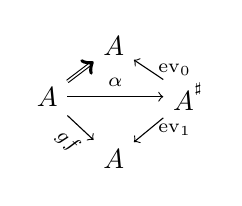
\begin{tikzpicture}[x=1.6em,y=1.4em]
  \node (At) at (1.5,2.4) {$A$};
  \node (Al) at (0,1.1) {$A$};
  \node (M) at (3.2,1.1) {$A^{\qcInt^{\sharp}}$};
  \node (Ab) at (1.5,-0.5) {$A$};
  \draw[double,->] (Al) -- (At);
  \draw[->] (Al) -- node[above]{$\scriptstyle\alpha$} (M);
  \draw[->] (M) -- node[right]{$\scriptstyle\mathrm{ev}_{0}$} (At);
  \draw[->] (M) -- node[right]{$\scriptstyle\mathrm{ev}_{1}$} (Ab);
  \draw[->] (Al) -- node[below,sloped]{$\scriptstyle gf$} (Ab);
\end{tikzpicture}
\qquad 与 \qquad
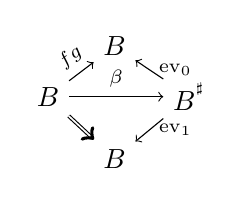
\begin{tikzpicture}[x=1.6em,y=1.4em]
  \node (Bt) at (1.5,2.4) {$B$};
  \node (Bl) at (0,1.1) {$B$};
  \node (M) at (3.2,1.1) {$B^{\qcInt^{\sharp}}$};
  \node (Bb) at (1.5,-0.5) {$B$};
  \draw[->] (Bl) -- node[above,sloped]{$\scriptstyle fg$} (Bt);
  \draw[->] (Bl) -- node[above]{$\scriptstyle\beta$} (M);
  \draw[->] (M) -- node[right]{$\scriptstyle\mathrm{ev}_{0}$} (Bt);
  \draw[->] (M) -- node[right]{$\scriptstyle\mathrm{ev}_{1}$} (Bb);
  \draw[double,->] (Bl) -- (Bb);
\end{tikzpicture}
\end{center}
反之，这样一份数据经限制便展现出一个复状单纯集的\trEquivalence。
\end{corollary}

\begin{proof}
\cref{def:complicial-equivalences}的数据可以提升如下：
\begin{center}
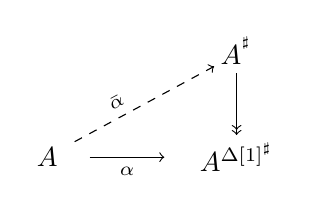
\begin{tikzpicture}[x=1.8em,y=1.6em]
  \node (m) at (3.8,1.2) {$A^{\qcInt^{\sharp}}$};
  \node (bl) at (0,-1.2) {$A$};
  \node (br) at (3.8,-1.2) {$A^{\Delta[1]^{\sharp}}$};
  \draw[->,dashed] (0.55,-0.85) -- node[above,sloped,pos=0.35]{$\scriptstyle\bar{\alpha}$} (3.35,0.85);
  \draw[->>] (3.8,0.7) -- (3.8,-0.7);
  \draw[->] (0.85,-1.2) -- node[below]{$\scriptstyle\alpha$} (2.35,-1.2);
\end{tikzpicture}
\qquad
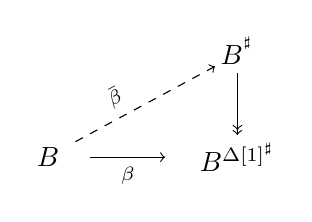
\begin{tikzpicture}[x=1.8em,y=1.6em]
  \node (m) at (3.8,1.2) {$B^{\qcInt^{\sharp}}$};
  \node (bl) at (0,-1.2) {$B$};
  \node (br) at (3.8,-1.2) {$B^{\Delta[1]^{\sharp}}$};
  \draw[->,dashed] (0.55,-0.85) -- node[above,sloped,pos=0.35]{$\scriptstyle\bar{\beta}$} (3.35,0.85);
  \draw[->>] (3.8,0.7) -- (3.8,-0.7);
  \draw[->] (0.85,-1.2) -- node[below]{$\scriptstyle\beta$} (2.35,-1.2);
\end{tikzpicture}
\end{center}
\end{proof}

我们想对\trQuasiCategory{}之间的\trIsofibration{}证明与
\cref{cor:leibniz-exponential}(iii) 与 (iv) 类比的命题，这需要与
\cref{prop:leibniz-marked-anodyne}及\cref{cor:leibniz-anodyne}类比的命题，
用以分析\trSimplicialSet{}的诸\trMonomorphism{}与包含
$\qcOne\hookrightarrow\qcInt$ 的\trLeibnizProduct。我们将通过考察%
\trQuasiCategory{}中的\trIsomorphism{}与复状单纯集中带标记边之间的关系
来推导这一点——这正是下一节的主题。

\subsection*{练习}

\begin{exercise}\label{ex:unmarked-leibniz-corollary}
陈述并证明\cref{cor:leibniz-mono-tf}的非带标记类比。
\end{exercise}

\begin{exercise}\label{ex:regular-entire-leibniz-products}
一个正则包含与一个非可逆的\trEntireInclusion{}的\trLeibnizProduct{}是\trEntireInclusion，但未必是正则包含。
找出展现这两种可能性的例子，并对那些必然正则的此类\trLeibnizProduct{}陈述并证明
一个刻画。这原本会简化\cref{prop:leibniz-marked-anodyne}的证明吗？
\end{exercise}

\begin{exercise}\label{ex:restriction-map-equivalence}
若 $f\colon X\to Y$ 是一个带标记\trHomotopyEquivalence{}而 $A$ 是一个复状
单纯集，证明：限制映射 $f^{*}\colon A^{Y}\to A^{X}$ 是复状单纯集间的一个%
\trEquivalence。
\end{exercise}

